\documentclass{standalone}

\usepackage[OT1]{fontenc}
\renewcommand*\familydefault{\sfdefault}
\usepackage{helvet,sfmath}
\usepackage{siunitx}

\usepackage{tikz}
\usetikzlibrary{arrows,calc,patterns}
% \usetikzlibrary{intersections, calc, arrows.meta}
\usepackage{tikz,tkz-euclide}

\begin{document}

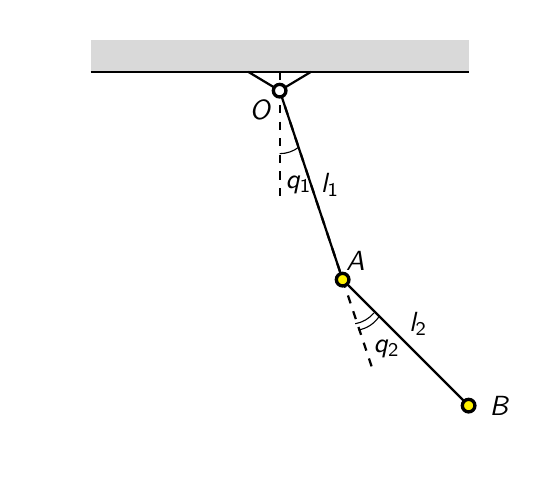
\begin{tikzpicture}[scale=0.8]
    %%Background
    \draw[draw=none] (-4,1) rectangle (4,-6);

    %%Ground
    \draw[draw=none, fill = gray!30] (-3,0.3) rectangle (3,0.8);
    \draw[thick] (-3,0.3) to (3,0.3);
    \draw[thick] (0.5,0.3) to (0,0);
    \draw[thick] (-0.5,0.3) to (0,0);

    %%Pendulum
    \draw[thick] (0,0) to (1,-3) to (3,-5);

    \draw[thick, dashed] (0,0.3) to (0,-1.8);
    % \draw[thick, dashed] (1,-2.5) to (1,-4.8);
    \draw[thick, dashed] (0,0) to (1.5,-4.5);
    
    \filldraw[color=black, fill=white, very thick] (0,0) circle (0.1);
    \filldraw[color=black, fill=yellow, very thick] (1,-3) circle (0.1);
    \filldraw[color=black, fill=yellow, very thick] (3,-5) circle (0.1);

    %% Angle
    \draw (0,-1) arc (270:308:0.5);
    \draw (1.2,-3.7) arc (280:320:0.5);
    \draw (1.25,-3.8) arc (280:325:0.5);
    
    %% Note
    \draw
    (-0.3,-0.3) node{\(O\)}
    (1.2,-2.7) node{\(A\)}
    (3.5,-5) node{\(B\)}
    (0.3,-1.5) node{\(q_1\)}
    (1.7,-4.1) node{\(q_2\)}
    (0.8,-1.5) node{\(l_1\)}
    (2.2,-3.7) node{\(l_2\)}
    ;

    
\end{tikzpicture}

\end{document}
